\documentclass[12pt]{article}
\usepackage[english]{babel}
\usepackage{float}
\usepackage[margin=1in]{geometry}
\usepackage{graphicx}
%\usepackage[toc,page]{appendix}
\graphicspath{ {./img/} }
\newcommand{\rpm}{\raisebox{.2ex}{$\scriptstyle\pm$}} 
\usepackage{listings}
\usepackage{xcolor}
\usepackage{indentfirst}
\usepackage{caption}
\usepackage[final]{pdfpages}
\usepackage{amsmath}
\usepackage[normalem]{ulem}

%# 16-833 SLAM Homework 3
%# Joe Phaneuf ( andrew id: jphaneuf)
%# March 29 2018
%## Collaborators : Adam Driscoll (jdriscol) , David Evans ( dje1 )  


\begin{document}

\title{Joe Phaneuf \\ Computer Vision 16-720 Spring 2018 Homework 5 \\ Apr. 11 2018 }
\date{}
\author{}
\maketitle

\newpage


\stepcounter{section}
%%%%%%%%%%%%%%%%%%%%%%%%%%%%%%%%%%%%%%%%%%%%%%%%%%%%%%%%%%%%%%%%%%%%%%%%%%%%%%%%
%%%%%%%%%%%%%%%%%%%%%%%%%%%%%%%%%%%%%%%%%%%%%%%%%%%%%%%%%%%%%%%%%%%%%%%%%%%%%%%%
\section{}
\subsection{a}
Point-to-point Iterative Closest Point defines an energy function to minimize in terms of Euclidean distance between a point, and a point at a subsequent timestep having undergone some transformation. This yields an estimate of the transformation. 

Point-to-plane Iterative Closest Point defines an energy function to minimize the dot product of a normal vector estimate and the difference between a vertex and a transformed vertex at a subsequent timestep. This also yields an estimate of the transformation, with an emphasis on maintaining surfaces.

\subsection{b}
So, we would like to estimate $\tilde{T}_{g,k}$, which transforms points in the camera frame to the world frame, and consequently provides camera pose.  
To estimate this new transform, we compute multiple iterations of small changes to the transform and solve for a gradient at each iteration. So, we need the incremental transform in solveable form!

At each iteration z, define $\tilde{T}_{inc}^{z}$ such that 
\begin{equation}
\tilde{T}_{g,k}^{z} = \tilde{T}_{inc}^{z} \tilde {T}_{g,k}^{z-1}
\end{equation}  
  
$\tilde{T}_{inc}^{z}$ contains a rotation and tanslation in 3 dimensions. Using the small angle approximation, we can approximate the rotation component as
\begin{equation}
\tilde{R}^{z} = 
\begin{bmatrix}
1 & \alpha & - \gamma \\
- \alpha & 1 & \beta \\
\gamma & - \beta & 1
\end{bmatrix}
\end{equation}
  
and the transformation component as
\begin{equation}
\tilde{t}^{z} = 
\begin{bmatrix}
tx \\ ty \\ tz
\end{bmatrix}
\end{equation}
  
We'll set up the minimization by equating the current frame transform estimate applied to a camera frame vertex to the incremental transform applied to a world frame vertex.
\begin{equation}
\tilde{T}_{g,k}^{z} \dot{V}_{k}= \tilde{R}^{z} \tilde{V}_{k}^{g}(u) + \tilde{t}^{z}
\end{equation}
  
Say that $\tilde{V}_{k}^{g}(u) = \begin{bmatrix} v_{1} & v_{2} & v_{3} \end{bmatrix}^{T}$
  
Then
\begin{equation}
\tilde{T}_{g,k}^{z} \dot{V}_{k}=
\begin{bmatrix}
         v_{1} +   \alpha v_{2} + - \gamma v_{3} \\
- \alpha v_{1} +          v_{2} +   \beta  v_{3}\\
  \gamma v_{1} + - \beta  v_{2} +          v_{3}
\end{bmatrix}
+ 
\tilde{t}^{z}  =
\begin{bmatrix}
            0  +   \alpha v_{2} -   \gamma v_{3} \\
- \alpha v_{1} +             0  +   \beta  v_{3} \\
  \gamma v_{1} -   \beta  v_{2} +             0
\end{bmatrix}
+ 
\begin{bmatrix} v_{1} \\ v_{2} \\ v_{3} \end{bmatrix} +
\tilde{t}^{z}  =
\end{equation}
\begin{equation}
\begin{bmatrix}
            0  - \gamma v_{3} + \alpha v_{2}  \\
  \beta  v_{3} +           0  - \alpha v_{1}  \\
- \beta  v_{2} + \gamma v_{1} +           0
\end{bmatrix}
+ 
\begin{bmatrix} v_{1} \\ v_{2} \\ v_{3} \end{bmatrix} +
\tilde{t}^{z}
=
\begin{bmatrix} \tilde{V}_{k}^{g}(u) \end{bmatrix}_{x} \begin{bmatrix} \beta \\ \gamma \\ \alpha \end{bmatrix}
+ 
\begin{bmatrix} v_{1} \\ v_{2} \\ v_{3} \end{bmatrix} +
\tilde{t}^{z}  =
\end{equation}
\begin{equation}
\left[
\begin{array}{cc}
\begin{bmatrix} \tilde{V}_{k}^{g}(u) \end{bmatrix}_{x} | & I 
\end{array}
\right]
\begin{bmatrix} \beta \\ \gamma \\ \alpha \\ tx \\ ty \\ tz \end{bmatrix} +
\tilde{V}_{k}^{g}(u)
\end{equation}

This is neat, because the incremental transform parameters can now be solved with linear solving tools.

\subsection{}
Figures \ref{fig:2dview1}, \ref{fig:2dview2}, and \ref{fig:2dview3} show three views of the reconstructed trajectory of camera poses using the iterative closest point algorithm. The trajectory breaks shortly after the first frame, but recovers a clean looking estimate over the remaining frames.


\begin{figure}[H]
\centering
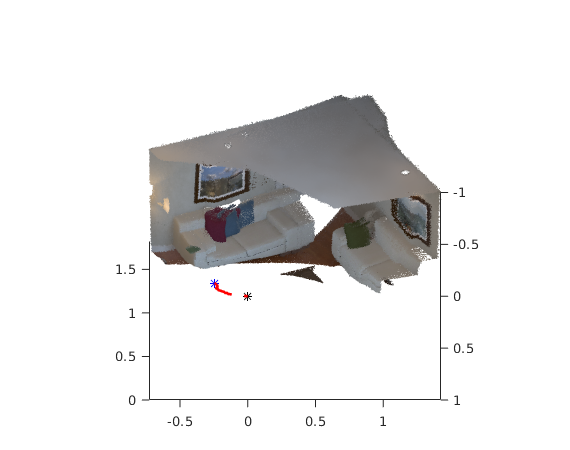
\includegraphics[page=1,width=0.75\textwidth]{2d_view1}
\caption{ ICP Trajectory View 1 } 
\label{fig:2dview1}
\end{figure}   

\begin{figure}[H]
\centering
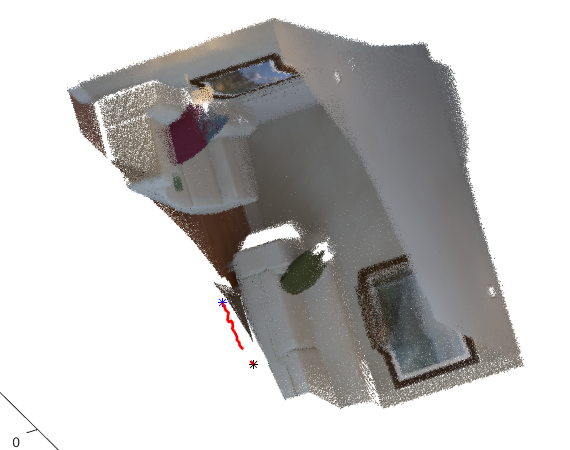
\includegraphics[page=1,width=0.75\textwidth]{2d_view2}
\caption{ ICP Trajectory View 2 } 
\label{fig:2dview2}
\end{figure}   

\begin{figure}[H]
\centering
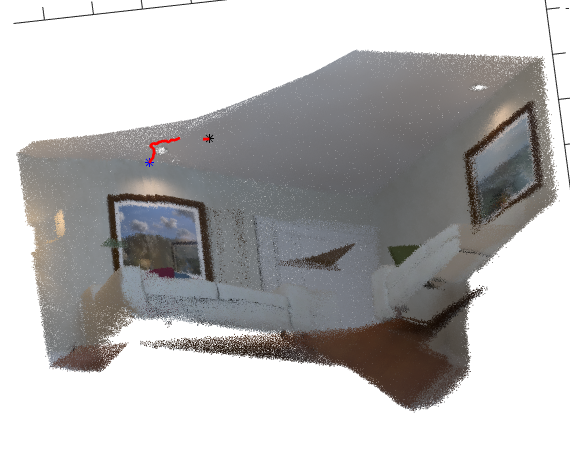
\includegraphics[page=1,width=0.75\textwidth]{2d_view3}
\caption{ ICP Trajectory View 3 } 
\label{fig:2dview3}
\end{figure}   

\section{}
\subsection{a}
Volumetric fusion methods suffer from high computational cost, and high memory requirements for Voxel grid storage as compared to point-based fusion methods.
\subsection{b}
Consider a point $p$ mapped into a new frame to point $p'$ by rotation $R$ and translation $t$.
\begin{equation}
p = R p + t
\end{equation}
  
The point's corresponding normal vector $n$ is mapped to the new frame by

\begin{equation}
n' = R n
\end{equation}

\subsection{d}
Figures \ref{fig:fusion1}, \ref{fig:fusion2}, and \ref{fig:fusion3} show three views of the resulting fused pointcloud obtained from point-based fusion. The fused map looks good! It contains  approximately three times as many points as a single input pointcloud, but does not appear to have any inconsistencies or warp. Interestingly, the resulting camera pose trajectories look better than with the previous fusion method.

\begin{figure}[H]
\centering
\includegraphics[page=1,width=0.75\textwidth]{fusion_view1}
\caption{ Fusion Map View 1 } 
\label{fig:fusion1}
\end{figure}   

\begin{figure}[H]
\centering
\includegraphics[page=1,width=0.75\textwidth]{fusion_view2}
\caption{ Fusion Map View 2 } 
\label{fig:fusion2}
\end{figure}   

\begin{figure}[H]
\centering
\includegraphics[page=1,width=0.75\textwidth]{fusion_view3}
\caption{ Fusion Map View 3 } 
\label{fig:fusion3}
\end{figure}   

\section{}
\subsection{a}
Comparing trajectories between the camera pose trajectories in the previous two sections, using the fusion model as the next reference frame results in much better ICP registration. This is because the fusion map provides a more stable reference with each consecutive iteration as points are added and updated.
\subsection{b}


\end{document}


